% TikZ coverage: scripts/texbundle.mjs compiles this and ships the files TeX
% reads, so decks can \usepackage{tikz} with these libraries. Add here
% whatever TikZ should support.
\documentclass{nicrainha}
\usepackage{tikz}
\usetikzlibrary{arrows.meta, calc, positioning, shapes.geometric, shapes.misc,
  decorations.pathreplacing, decorations.markings, backgrounds, fit,
  intersections, patterns, matrix, shadings, through}
\begin{document}
\begin{slide}{Paths and nodes}
  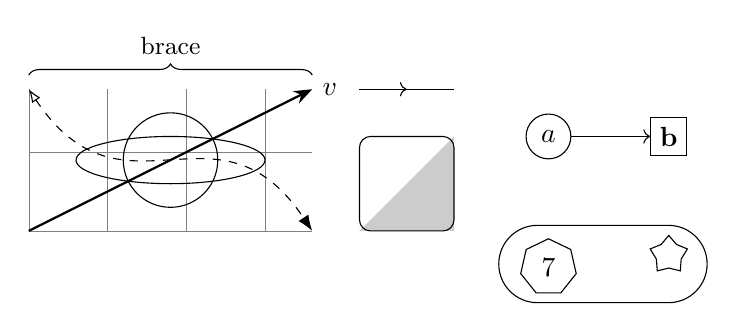
\begin{tikzpicture}[x=6mm, y=6mm]
    \draw[help lines] (0, 0) grid (6, 3);
    \draw[-Stealth, thick] (0, 0) -- (6, 3) node[right] {$v$};
    \draw[{Latex[open]}-{Latex[length=2mm]}, dashed] (0, 3) .. controls (2, 0) and (4, 3) .. (6, 0);
    \draw (3, 1.5) circle[radius=1] (3, 1.5) ellipse[x radius=2, y radius=0.5];
    \draw[rounded corners] (7, 0) rectangle (9, 2);
    \fill[fill opacity=0.2] (7, 0) -- (9, 2) -- (9, 0) -- cycle;
    \node[draw, circle] (a) at (11, 2) {$a$};
    \node[draw, rectangle, right=of a] (b) {\textbf{b}};
    \node[draw, regular polygon, regular polygon sides=7, below=of a] (c) {7};
    \node[draw, star, below=of b] (d) {};
    \node[draw, rounded rectangle, fit=(c) (d)] {};
    \draw[->] (a) -- (b);
    \draw[decorate, decoration={brace, amplitude=4pt}] (0, 3.3) -- node[above=4pt] {\small brace} (6, 3.3);
    \draw[postaction={decorate}, decoration={markings, mark=at position 0.5 with {\arrow{>}}}] (7, 3) -- (9, 3);
  \end{tikzpicture}
\end{slide}

\begin{slide}{Plots, loops, fills}
  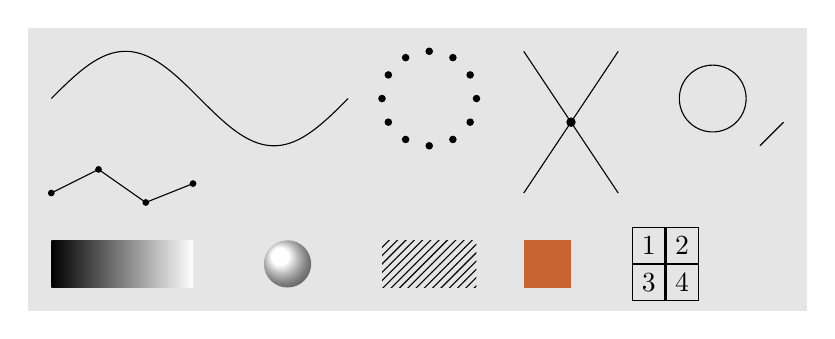
\begin{tikzpicture}[x=6mm, y=6mm]
    \draw[domain=0:6.283, samples=60, smooth] plot (\x, {sin(\x r)});
    \draw plot[mark=*, mark size=1pt] coordinates {(0, -2) (1, -1.5) (2, -2.2) (3, -1.8)};
    \foreach \k in {0, ..., 11} \fill ({8 + cos(30 * \k)}, {sin(30 * \k)}) circle[radius=0.08];
    \draw[name path=p] (10, -2) -- (12, 1);
    \draw[name path=q] (10, 1) -- (12, -2);
    \fill[name intersections={of=p and q}] (intersection-1) circle[radius=0.1];
    \shade[left color=black, right color=white] (0, -4) rectangle (3, -3);
    \shade[ball color=white] (5, -3.5) circle[radius=0.5];
    \fill[pattern=north east lines] (7, -4) rectangle (9, -3);
    \fill[color={rgb,255:red,200;green,100;blue,50}] (10, -4) rectangle (11, -3);
    \matrix[matrix of nodes, nodes={draw}] at (13, -3.5) {1 & 2 \\ 3 & 4 \\};
    \coordinate (o) at (14, 0);
    \node[draw] at (o) [circle through={(14.5, 0.5)}] {};
    \draw let \p1 = (o), \n1 = {veclen(\x1, \y1)} in (15, -1) -- +(0.5, 0.5);
    \begin{scope}[on background layer]
      \fill[fill opacity=0.1] (-0.5, -4.5) rectangle (16, 1.5);
    \end{scope}
  \end{tikzpicture}
\end{slide}
\end{document}
